% Slides for 2024-05-20
\begin{frame}{New Carousel Images}
    \begin{columns}
        \begin{column}{0.33\textwidth}
            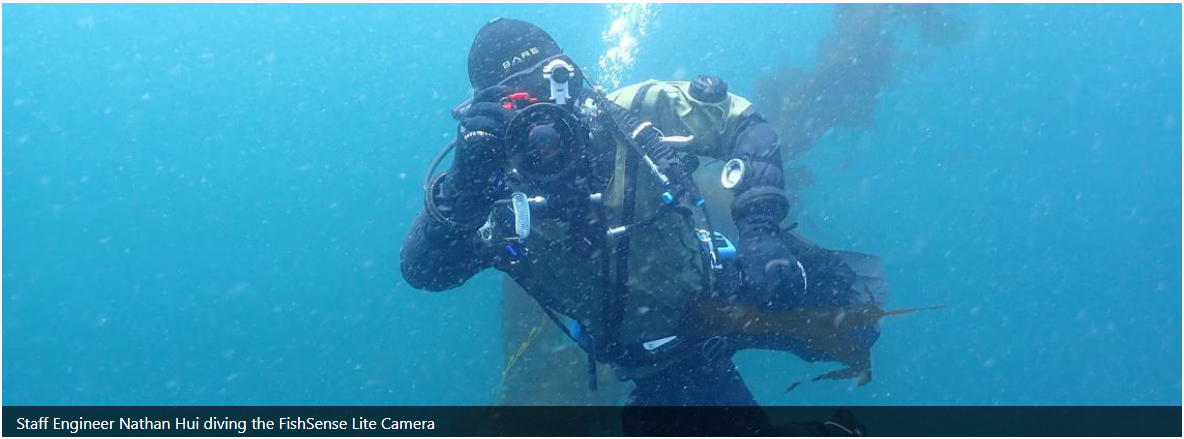
\includegraphics[width=\linewidth]{images/web_carousel_1.png}
            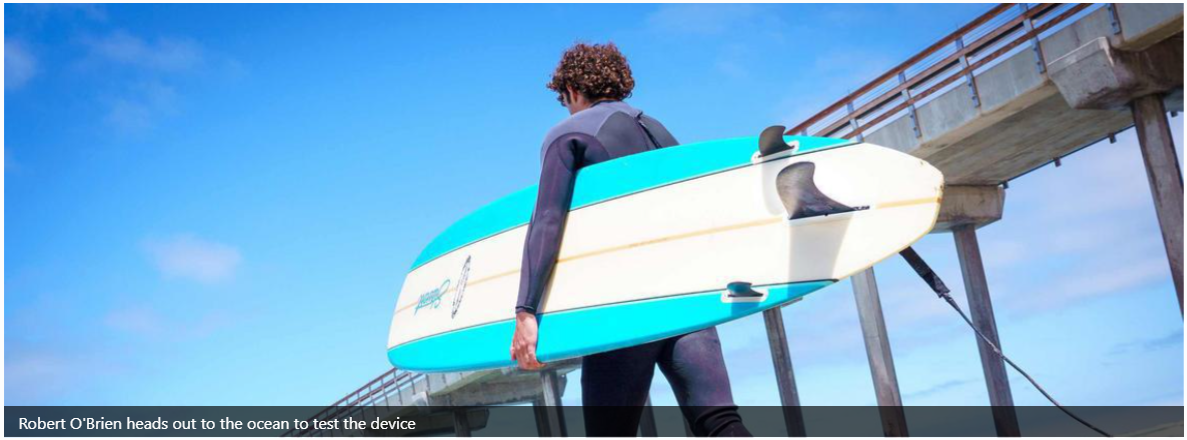
\includegraphics[width=\linewidth]{images/web_carousel_2.png}
            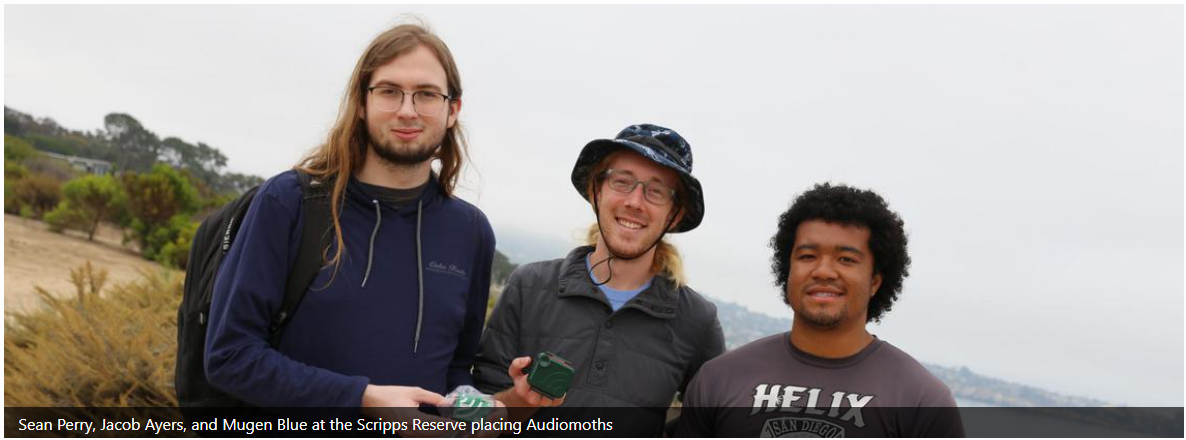
\includegraphics[width=\linewidth]{images/web_carousel_3.png}
        \end{column}
        \begin{column}{0.33\textwidth}
            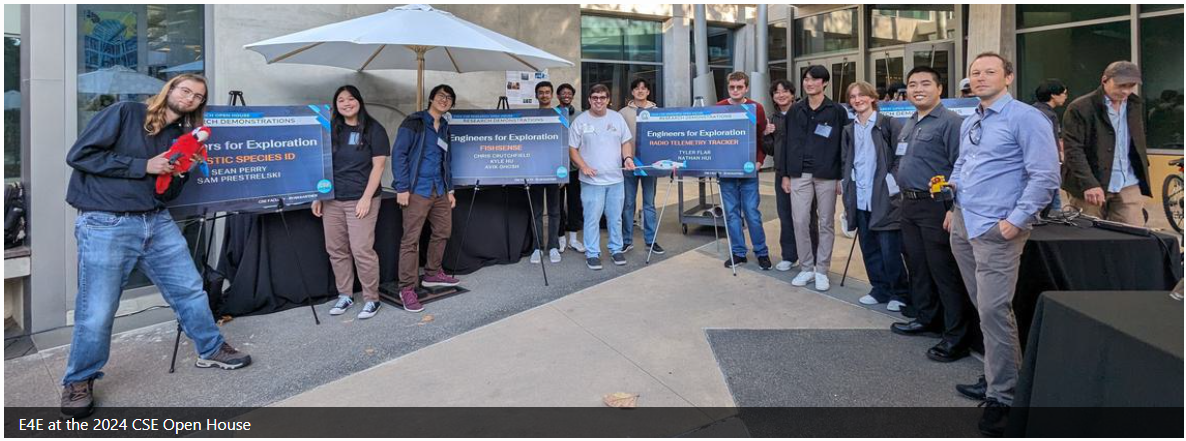
\includegraphics[width=\linewidth]{images/web_carousel_4.png}
            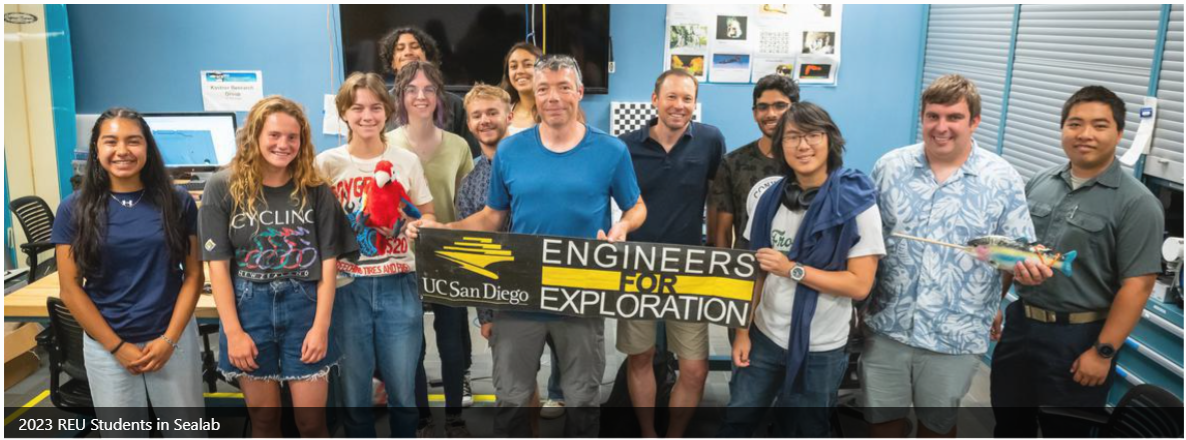
\includegraphics[width=\linewidth]{images/web_carousel_5.png}
            
\includegraphics[width=\linewidth]{images/web_carousel_6.png}
            
\includegraphics[width=\linewidth]{images/web_carousel_7.png}
        \end{column}
        \begin{column}{0.33\textwidth}
            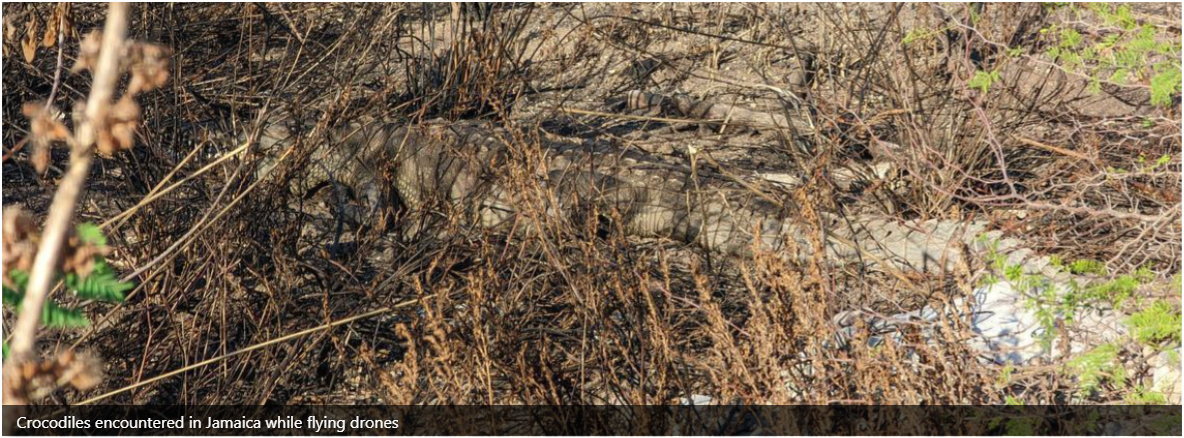
\includegraphics[width=\linewidth]{images/web_carousel_8.png}
            
\includegraphics[width=\linewidth]{images/web_carousel_9.png}
            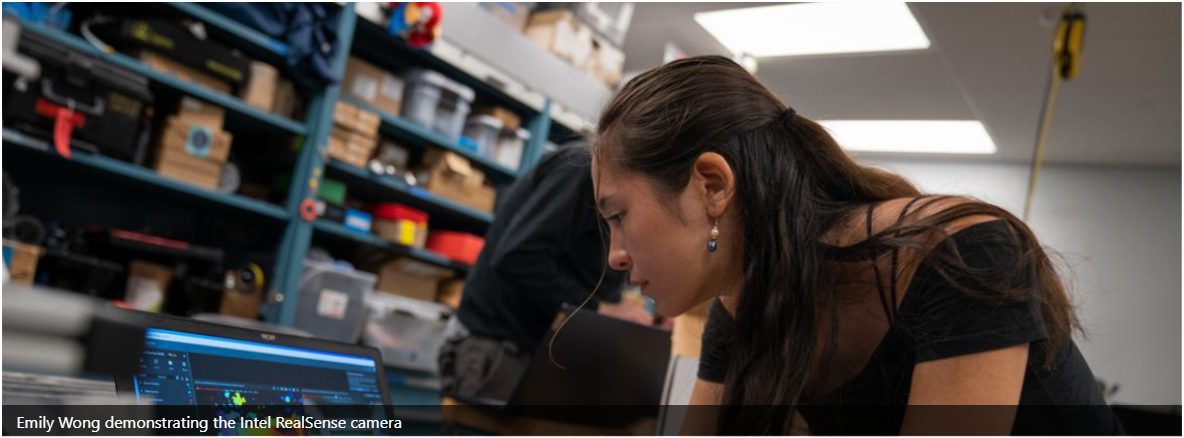
\includegraphics[width=\linewidth]{images/web_carousel_10.png}
        \end{column}
    \end{columns}
\end{frame}
\begin{frame}{Goal for Summer}
    One new carousel photo from each E4E project
\end{frame}

\begin{frame}{Add onboarding papers}
    \centering
    
\includegraphics[height=0.7\textheight,width=0.7\textwidth,keepaspectratio]{images/onboarding.png}
\end{frame}

\begin{frame}{WIP Homepage and archived}
    \begin{columns}
        \begin{column}{0.5\textwidth}
            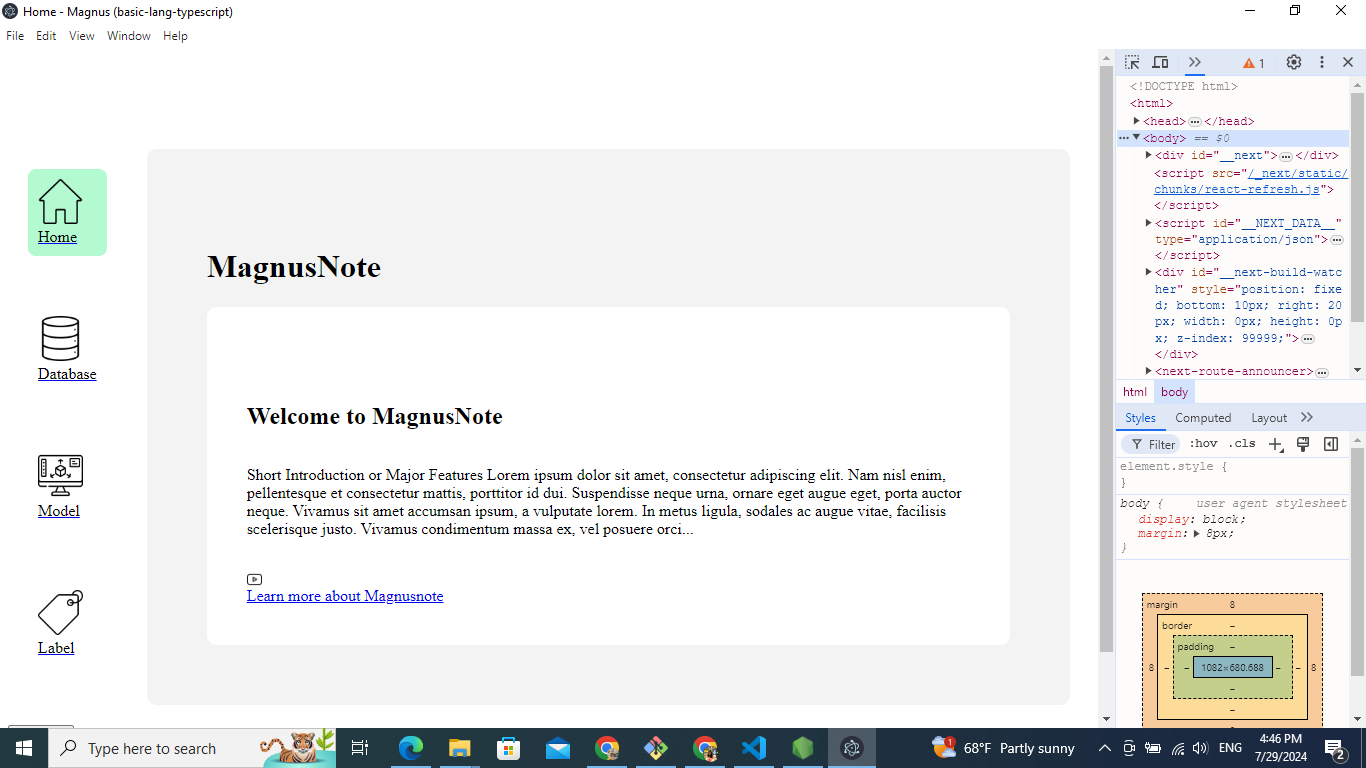
\includegraphics[width=\linewidth]{images/homepage.png}
        \end{column}
        \begin{column}{0.5\textwidth}
            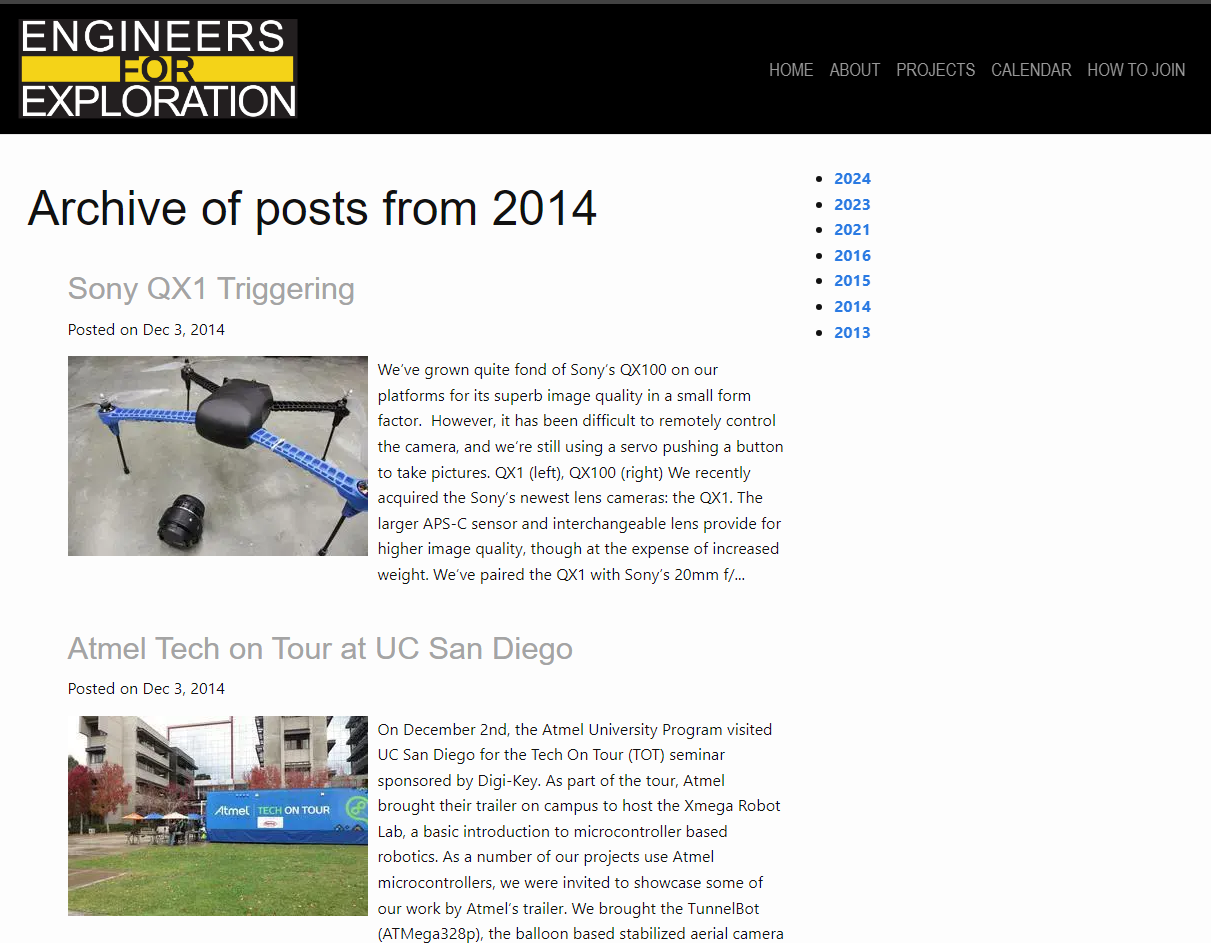
\includegraphics[width=\linewidth]{images/archive.png}
        \end{column}
    \end{columns}
\end{frame}

\begin{frame}{WIP People pages}
    \centering
    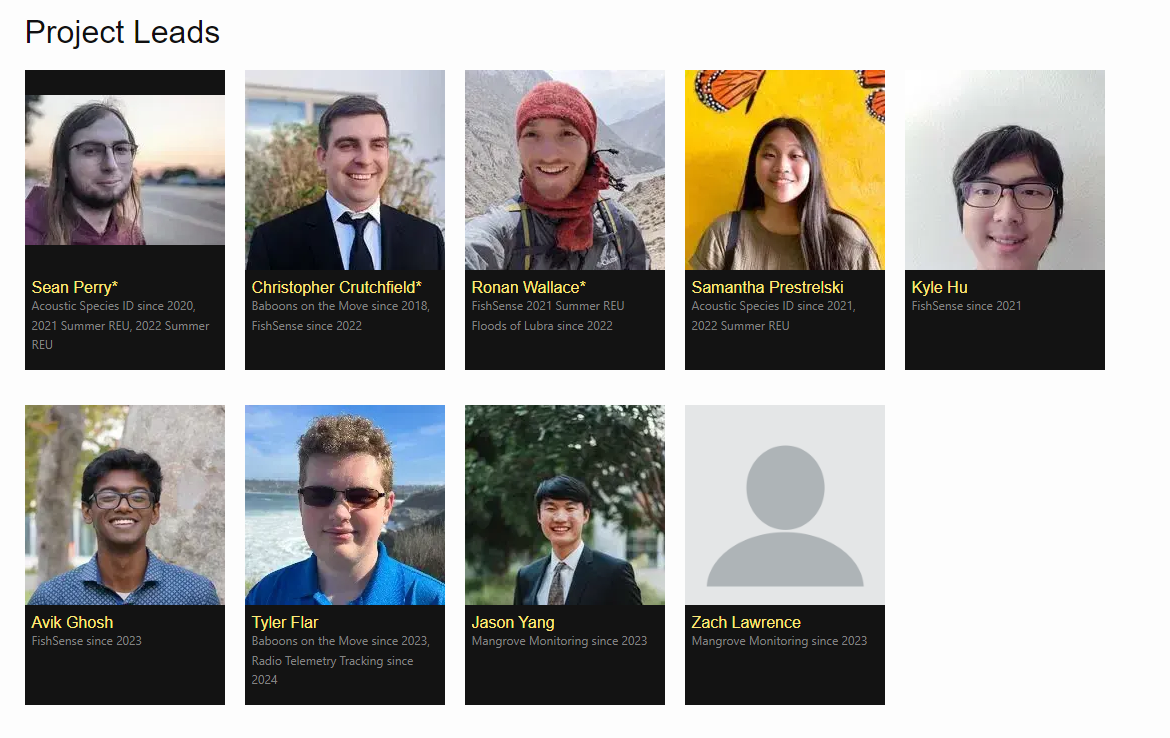
\includegraphics[height=0.7\textheight,width=0.7\textwidth,keepaspectratio]{images/People.png}
\end{frame}

\begin{frame}{Less Dramatic Updates}
    \begin{itemize}
        \item Foundation and gulp added
        \item WIP: link checker and image caching
        \item WIP: started building 2016 - 2017 posts
    \end{itemize}
\end{frame}

% To create a slide, use the following:
% \begin{frame}{TITLE}
%     BODY
% \end{frame}

% To create a slide with a bullet list, use the following:
% \begin{frame}{TITLE}
%     \begin{itemize}
%         \item ITEM 1
%         \item ITEM 2
%     \end{itemize}    
% \end{frame}

% To create a slide with numbered list, use the following:
% \begin{frame}{TITLE}
%     \begin{enumerate}
%         \item ITEM 1
%         \item ITEM 2
%     \end{enumerate}
% \end{frame}

% To create a slide with a graphic:
% 1. Add the graphic to this folder (named picture.png)
% 2. Use the following:
% \begin{frame}{TITLE}
%     \centering
%     \includegraphics[height=0.7\textheight,width=0.7\textwidth,keepaspectratio]{picture.png}
% \end{frame}

% To create a slide with two columns, use the following:
% \begin{frame}{TITLE}
%     \begin{columns}
%         \begin{column}{0.5\textwidth}
%             COLUMN 1 BODY
%         \end{column}
%         \begin{column}{0.5\textwidth}
%             COLUMN 2 BODY
%         \end{column}
%     \end{columns}
% \end{frame}
